% called by main.tex
\chapter{Cơ sở lý thuyết và thuật toán}
\label{ch::chapter2}
\section{Cơ sở lý thuyết}

CSMA/CA (Carrier Sense Multiple Access with Collision Avoidance) là một phương pháp truy cập truyền 
thông được sử dụng trong mạng không dây để giảm thiểu va chạm dữ liệu. Đây là một phương pháp truy 
cập ngẫu nhiên trong đó các thiết bị trong mạng truyền thông sẽ kiểm tra tình trạng kênh trước khi 
truyền dữ liệu và thực hiện các biện pháp để tránh xung đột dữ liệu.

Nguyên tắc cơ bản khi truy cập của chuẩn IEEE 802.11 là sử dụng cơ chế CSMA/CA– Đa truy cập sử dụng sóng 
mang phòng tránh xung đột. Nguyên tắc này gần giống như nguyên tắc CSMA/CD (Carrier Sense Multiple 
Access Collision Detect) của chuẩn 802.3 (cho Ethernet). Điểm khác ở đây là CSMA/CA nó sẽ chỉ truyền 
dữ liệu khi bên kia sẵn sàng nhận và không truyền hay nhận dữ liệu nào khác trong lúc đó, đây còn gọi 
là nguyên tắc LBT (listening before talking) – nghe trước khi nói.

Theo chuẩn IEEE 802.11, kỹ thuật CSMA/CA được sử dụng tại lớp MAC bởi hàm Distributed Coordination Function (DCF) như trong hình ~\ref{fig:mac}.
\begin{figure}[h]
    \centering
    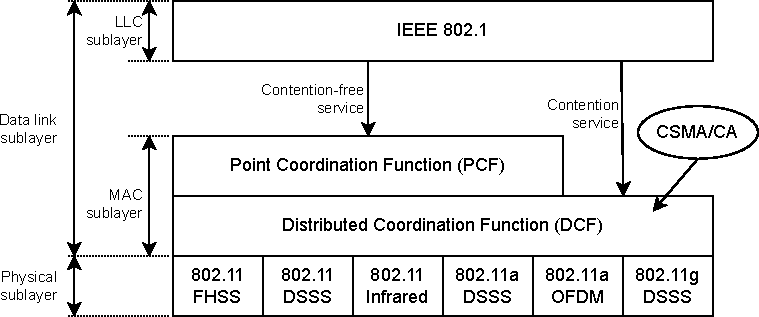
\includegraphics[width=0.65\linewidth]{figures/Chapter2/MAClayer_k2opt.pdf}
    %width=
    \caption{Lớp MAC trong chuẩn IEEE 802.11}
    \label{fig:mac}
\end{figure}
